\documentclass[11pt]{article}

\usepackage[margin=1in]{geometry}
\usepackage{booktabs}
\usepackage{array}
\usepackage{longtable}
\usepackage{hyperref}
\usepackage{xcolor}
\usepackage{tikz}
\usepackage{amsmath}
\usepackage{fancyhdr}
\usepackage{caption}
\usetikzlibrary{arrows.meta,positioning,shapes.geometric,fit}

\hypersetup{
  colorlinks=true,
  linkcolor=blue!60!black,
  urlcolor=blue!60!black,
  citecolor=blue!60!black
}

\pagestyle{fancy}
\setlength{\headheight}{14pt}
\fancyhf{}
\lhead{Universal Systems Compiler}
\rhead{Rangnekar and Phadke}
\cfoot{\thepage}

\newcommand{\motif}[1]{\textsc{#1}}
\newcommand{\code}[1]{\texttt{\detokenize{#1}}}
\newcolumntype{L}[1]{>{\raggedright\arraybackslash}p{#1}}
\setlength{\emergencystretch}{2em}

\title{\textbf{The Universal Systems Compiler and the Motif Atlas}\\
\large A Structural Intermediate Representation for Cross-Domain Invention}
\author{Nikit Phadke}
\date{June 2026}

\begin{document}
\maketitle

\begin{abstract}
A database engineer ensuring cache consistency, a molecular biologist studying
chromosome alignment during mitosis, and a diplomat mediating a border dispute
are solving the same structural problem: how do divergent copies arrive at a
consistent state under constraints? Their vocabularies differ, but the motif
structure is shared. This paper introduces the Universal Systems Compiler
(USC), a framework for parsing systems from any domain into a typed structural
intermediate representation based on a 32-motif atlas. The atlas separates
structure from domain metadata. Motifs act simultaneously as lexer tokens,
vector dimensions, graph node types, and semantic diagnostics. The compiler
builds motif ASTs, checks composition valence, detects impossible motif
collisions, audits implementation fidelity, and emits typed transfer contracts
for cross-domain pattern grafting. We report an executable prototype containing
an Atlas Kernel, motif2vec retrieval artifacts, a BioMotif compiler over EGFR,
a System2Vec bridge, and Bio AST execution contracts. The central claim is not
that analogy alone is safe. The central claim is that analogy becomes
engineering when it is constrained by motif valence, substrate mismatch audits,
and executable validation gates.
\end{abstract}

\section{Introduction}

Human knowledge is organized by substrate. Computer science, biology,
economics, law, psychology, and governance have separate languages,
institutions, journals, and intuitions. Yet many of their hardest problems have
the same structural form. Caches, chromosomes, ledgers, and diplomatic claims
all replicate, diverge, synchronize, and reconcile. Markets, immune systems,
and search engines all route feedback under scarcity into better
representations. Legislatures, cell nuclei, and operating systems all enforce
invariants through scoped authority.

The Universal Systems Compiler addresses this mismatch between substrate-bound
vocabulary and substrate-independent structure. It proposes a common structural
alphabet: the Motif Atlas. A motif is not a design pattern. A pattern is a
domain-specific answer, such as a mutex, market circuit breaker, DNA mismatch
repair mechanism, or constitutional court. A motif is the universal question
that such answers solve: boundary, authority, feedback, reconciliation,
scarcity, representation, and so on.

The USC compiles domain-specific descriptions into motif ASTs. These ASTs can
be diagnosed, embedded, searched, modified, and decompiled back into
domain-native designs. This makes cross-domain transfer explicit. The compiler
does not merely say that a protein hinge is ``like'' a traffic ramp meter. It
asks which motifs match, which valences are missing, which substrate
assumptions break, and what engineering bridge would make the transfer
admissible.

\section{Motifs}

A motif is a recurring structural concern that arises independently of physical
substrate. Each motif is identified by a question that any sufficiently complex
system must answer. A motif earns its place by passing five tests:

\begin{itemize}
  \item \textbf{Recognition}: experts in multiple domains recognize it.
  \item \textbf{Transfer}: understanding it in one domain helps reason in another.
  \item \textbf{Compression}: naming it collapses many phenomena into one concept.
  \item \textbf{Prediction}: its absence predicts observable failure modes.
  \item \textbf{Design}: asking whether it is addressed reveals missing structure.
\end{itemize}

In the compiler, motifs perform quadruple duty. They are lexer tokens, vector
dimensions, graph node types, and semantic analyzer rules. A motif vector can
therefore support retrieval, while the AST and ProcessIR layers support
reasoning.

\section{The Motif Atlas}

The atlas contains 32 primitive motifs grouped into six families. Table
\ref{tab:motifs} gives the compact form. Longer operational definitions are
implemented in the Atlas Kernel artifact.

\begin{longtable}{rL{0.2\linewidth}L{0.2\linewidth}L{0.45\linewidth}}
\caption{The 32-motif atlas.}
\label{tab:motifs}\\
\toprule
\# & Motif & Group & Fundamental question \\
\midrule
\endfirsthead
\toprule
\# & Motif & Group & Fundamental question \\
\midrule
\endhead
1 & State & Existence & What currently exists? \\
2 & Transition & Existence & How does it change? \\
3 & Invariant & Existence & What must remain true after every change? \\
4 & Identity & Existence & What makes each thing uniquely itself? \\
5 & Boundary & Existence & What separates inside from outside? \\
6 & Terminal State & Existence & When is it done? \\
7 & Decay & Existence & What degrades without maintenance? \\
8 & Storage & Persistence & Where does information persist? \\
9 & Addressing & Persistence & How do you find what you need? \\
10 & Replication & Persistence & Can multiple copies exist? \\
11 & Synchronization & Persistence & How do copies stay consistent? \\
12 & Representation & Intelligence & How is reality encoded? \\
13 & Feedback & Intelligence & How does outcome influence future transitions? \\
14 & Prediction & Intelligence & What happens next? \\
15 & Search & Intelligence & How do you find a valid path? \\
16 & Model & Intelligence & What internal simulation exists? \\
17 & Compression & Intelligence & How can less describe more? \\
18 & Optimization & Intelligence & What should improve? \\
19 & Explore/Exploit & Intelligence & Learn or use? \\
20 & Self-Reference & Intelligence & When does a system reference itself? \\
21 & Composition & Structure & How do pieces combine? \\
22 & Hierarchy & Structure & How do small things form larger things under direction? \\
23 & Modularity & Structure & What can change independently? \\
24 & Abstraction & Structure & What can be hidden? \\
25 & Emergence & Structure & How do micro-behaviors produce macro-properties? \\
26 & Scarcity & Allocation & What is limited? \\
27 & Queue & Allocation & Who waits? \\
28 & Scheduling & Allocation & Who gets resources next? \\
29 & Communication & Coordination & How does information move? \\
30 & Authority & Coordination & Who decides? \\
31 & Reconciliation & Coordination & How do divergent states converge? \\
32 & Negotiation & Coordination & How do competing interests reach agreement? \\
\bottomrule
\end{longtable}

\subsection{Boundary as Scope}

Boundary has a special syntactic role. It is the scope delimiter of the motif
AST. A boundary that contains internal structure opens a new AST scope, just as
a brace opens a lexical scope in a programming language. Containment edges run
vertically through these scopes. Communication edges run horizontally across
boundaries. Authority edges run downward from parent scopes to child scopes,
propagating invariants.

\section{Grammar}

Motifs are not independent atoms. They have composition rules, input valences,
and collision rules. This grammar is what prevents cross-domain transfer from
collapsing into unconstrained analogy.

\subsection{Composition Graph}

Some motifs are composites of other motifs. Table \ref{tab:composition}
summarizes the executable rules currently implemented in the Atlas Kernel.

\begin{table}[h]
\centering
\caption{Selected composition rules.}
\label{tab:composition}
\small
\begin{tabular}{L{0.22\linewidth}L{0.38\linewidth}L{0.28\linewidth}}
\toprule
Composite & Requires & Provides \\
\midrule
Prediction & Representation, Feedback & Anticipation \\
Model & Representation, Prediction, Boundary & Counterfactual simulation \\
Compression & Representation, Scarcity & Generalization \\
Optimization & Prediction, Search, Scarcity & Directed improvement \\
Hierarchy & Composition, Authority & Directed scale \\
Modularity & Boundary, Composition & Independent change \\
Abstraction & Boundary, Representation & Interface hiding \\
Emergence & Composition, Feedback & Macro behavior \\
Queue & Scarcity, Composition & Visible waiting \\
Scheduling & Queue, Authority & Priority over time \\
Reconciliation & Communication, Invariant, Authority & Divergence resolution \\
Negotiation & Communication, Scarcity, Authority & Agreement under conflict \\
\bottomrule
\end{tabular}
\end{table}

\subsection{Motif Valence}

Each motif has prerequisites. If a system claims a motif without its
prerequisites, the compiler emits \code{MIRACLE}. For example,
Reconciliation requires Communication, Authority, and Invariant. Feedback
requires State, Transition, and Communication. Authority requires Boundary and
Invariant. These rules make transfer typed rather than impressionistic.

\subsection{Collisions}

Some motif combinations are impossible or pathological in any substrate. The
current kernel includes a halting-style collision:
Prediction, Self-Reference, and Terminal State. It also treats unscoped
Authority as an authority/boundary contradiction. The collision registry is
expected to grow as the atlas is tested against more domains.

\section{Physics: FEP Grounding}

The Free Energy Principle (FEP) proposes that self-organizing systems can be
understood as minimizing surprise or prediction error under a generative model
\cite{friston2010}. The motif atlas reaches a similar architecture from
structural assumptions rather than variational calculus.

Assume a persistent system has State, Boundary, Decay, and Scarcity. Because it
decays, it must Transition to maintain itself. Because resources are scarce, it
must use Feedback to determine whether transitions work. Feedback refines
Representation. Representation refined by Feedback enables Prediction.
Prediction bounded by Boundary enables Model. When model and feedback diverge,
the system can update representation or act through search and transition. The
former resembles perceptual inference; the latter resembles active inference.

The correspondence is not asserted as a replacement for FEP. It is a structural
cross-check. Two different formalisms converge on a viability core: State,
Boundary, Transition, and Feedback. The USC calls this the FEP viability check.

\section{Geometry: Motif Space}

Every system has a coordinate in 32-dimensional motif space. This coordinate is
lossy but useful. It discards full AST structure and preserves which motifs are
present and how strongly. The vector supports nearest-neighbor search across
domains. Systems close in motif space often share structural needs even when
their vocabulary is unrelated.

Empty regions of motif space are possible inventions. A region populated in
one domain but sparse in another marks a transfer opportunity. If finance has
high-fidelity feedback/authority throttles, while pharmacology has static
allosteric wedges, motif distance can expose the fidelity gap.

\section{The Compiler Architecture}

The compiler separates deterministic law from heuristic discovery.

\begin{figure}[h]
\centering
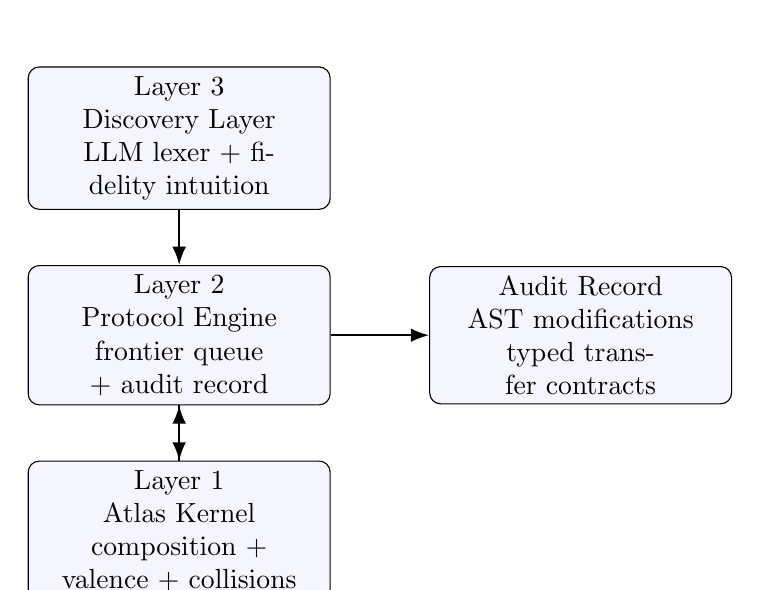
\begin{tikzpicture}[
  node distance=0.7cm,
  box/.style={draw, rounded corners, align=center, text width=3.6cm, minimum height=0.85cm, fill=blue!4},
  arr/.style={-Latex, thick}
]
\node[box] (l3) {Layer 3\\Discovery Layer\\LLM lexer + fidelity intuition};
\node[box, below=of l3] (l2) {Layer 2\\Protocol Engine\\frontier queue + audit record};
\node[box, below=of l2] (l1) {Layer 1\\Atlas Kernel\\composition + valence + collisions};
\node[box, right=1.25cm of l2] (out) {Audit Record\\AST modifications\\typed transfer contracts};
\draw[arr] (l3) -- (l2);
\draw[arr] (l2) -- (l1);
\draw[arr] (l1) -- (l2);
\draw[arr] (l2) -- (out);
\end{tikzpicture}
\caption{Three-layer USC architecture. Stochastic discovery is constrained by a deterministic kernel.}
\end{figure}

\subsection{Lexer}

The lexer reads domain-specific descriptions and emits motif tokens. It strips
metadata and preserves structure. For example, ``the compliance department
audits transactions'' becomes a scoped structure involving Invariant,
Feedback, Authority, and Boundary.

\subsection{Parser}

The parser builds an AST using Boundary nesting. Nodes carry motif signatures.
Edges are typed as containment, communication, or authority. Parent invariants
propagate downward unless a child adds stricter local invariants.

\subsection{Semantic Analysis}

The semantic analyzer runs composition completeness, valence checking,
invariant propagation, FEP viability, and collision detection. It does not
reject invalid real systems. Reality executes invalid systems anyway. The
compiler annotates the dysfunction.

\subsection{Engineering Audit}

Nodes that pass theoretical checks receive a three-test gate:
Coverage, Fidelity, and Stress. Coverage asks whether all required motifs are
present. Fidelity asks whether the implementation is structurally rich or
impoverished compared with nearby high-fidelity patterns. Stress asks whether
the implementation's physical assumptions survive scale, latency, adversaries,
noise, and substrate mismatch.

\section{Representations}

The USC uses three representations.

\begin{table}[h]
\centering
\caption{The three representations.}
\small
\begin{tabular}{L{0.2\linewidth}L{0.35\linewidth}L{0.32\linewidth}}
\toprule
Representation & Purpose & What it discards \\
\midrule
Vector & Retrieval and similarity search in 32-D motif space & AST topology and local bindings \\
Pattern & Transferable substrate-independent subgraph & Domain-specific vocabulary and physical substrate \\
AST & Diagnosis, modification, and code generation & Nothing essential for the local system \\
\bottomrule
\end{tabular}
\end{table}

The AST diagnoses. The vector searches. The pattern transfers. The modified
AST receives the graft and is rechecked.

\section{Cross-Domain Invention}

The isomorphic compilation pipeline contains five steps:

\begin{enumerate}
  \item \textbf{Extract}: isolate a broken node or desired motif vector.
  \item \textbf{Search}: query System2Vec for high-fidelity patterns.
  \item \textbf{Filter}: complete a typed transfer contract with substrate mismatches.
  \item \textbf{Graft}: instantiate the pattern at a valence-compatible point.
  \item \textbf{Decompile}: translate the modified motif logic into target-domain output.
\end{enumerate}

The filter step is essential. It prevents the compiler from accepting a
transfer merely because cosine similarity is high.

\section{Executable Prototype}

The repository contains a working prototype. Table \ref{tab:artifacts}
summarizes the major artifacts.

\begin{table}[h]
\centering
\caption{Executable USC artifacts.}
\label{tab:artifacts}
\footnotesize
\begin{tabular}{L{0.42\linewidth}L{0.44\linewidth}}
\toprule
Artifact & Role \\
\midrule
\code{experiments/usc_atlas_kernel.ts} & Deterministic Layer-1 kernel: motifs, composition graph, valence, collisions, FEP viability, and three-test gate. \\
\code{experiments/motif2vec_dataset.ts} & Generates a 10k motif2vec corpus and retrieval pairs. \\
\code{experiments/motif2vec_train.ts} & Trains a no-dependency 32-D motif regressor baseline. \\
\code{experiments/bio_motif_compiler.ts} & Compiles UniProt, Reactome, and AlphaFold data into BioMotifIR. \\
\code{experiments/system2vec_bio_bridge.ts} & Retrieves cross-domain control patterns for biological motif targets. \\
\code{experiments/bio_ast_execution_contract.ts} & Emits molecule-generator-facing AST execution contracts with safety gates. \\
\bottomrule
\end{tabular}
\end{table}

\subsection{Kernel Audit Result}

The kernel caught an important failure during development: a market volatility
circuit breaker claimed Prediction without explicitly sourcing Representation.
After adding Representation, the pattern received \code{TRUST}. Static
allosteric wedges and the EGFR transfer contracts remained guarded as
\code{MIRACLE} until missing biological valences are supplied.

\begin{table}[h]
\centering
\caption{Representative Atlas Kernel audit.}
\small
\begin{tabular}{L{0.32\linewidth}L{0.14\linewidth}L{0.37\linewidth}}
\toprule
Node & Verdict & Missing prerequisites \\
\midrule
Market volatility circuit breaker & TRUST & None \\
Static allosteric wedge & MIRACLE & Feedback requires State; Authority requires Invariant \\
EGFR 688-704 debounce contract & MIRACLE & Feedback requires State and Transition; Authority requires Invariant; Modularity and Hierarchy require Composition \\
\bottomrule
\end{tabular}
\end{table}

\subsection{BioMotif and System2Vec Case Study}

The BioMotif compiler was run on EGFR, UniProt accession P00533. It used
UniProt annotations, Reactome pathway mappings, and an AlphaFold predicted
structure. These open resources are well-established: Reactome is an
open-source curated pathway knowledgebase \cite{reactome2024}, AlphaFold DB
provides predicted structures \cite{alphafold2021}, and UniProt provides
programmatic protein annotations \cite{uniprot2023}.

The compiler identified an EGFR region annotated as important for dimerization,
phosphorylation, and activation, residues 688-704. Its motif signature included
Communication, Feedback, Authority, Modularity, and Hierarchy. System2Vec
retrieved richer control patterns:

\begin{table}[h]
\centering
\caption{System2Vec matches for EGFR residues 688-704.}
\small
\begin{tabular}{L{0.44\linewidth}rL{0.32\linewidth}}
\toprule
Pattern & Similarity & Transfer prescription \\
\midrule
Circuit breaker & 0.8147 & Stabilize a reversible safety boundary under pathological feedback. \\
Market volatility circuit breaker & 0.7703 & Prefer use-dependent binding to high-frequency transition states. \\
Bulkhead isolation & 0.7438 & Constrain propagation across modular signaling surfaces. \\
Ramp metering & 0.6898 & Gate engagement using downstream environmental context. \\
Debounce filter & 0.6847 & Suppress transient contacts while preserving sustained signaling. \\
\bottomrule
\end{tabular}
\end{table}

The execution contract does not claim a therapy. It emits a design hypothesis:
a context-aware, kinetic-gated allosteric modulator should avoid static
friction, prefer transition-like hinge conformations, remain weak in healthy
contexts, and activate only when both a conformational trigger and a
disease-context environmental gate are satisfied. The contract explicitly
requires docking, contact maps, selectivity checks, structural validation,
signaling assays, and toxicity testing before any scientific or medical claim.

\section{Relation to Prior Work}

The USC is adjacent to several traditions. Design patterns showed that
software designs can be cataloged as reusable structures \cite{gamma1994}.
Causal modeling made causal structure mathematically explicit \cite{pearl2009}.
The Free Energy Principle provided a general theory of adaptive
self-organization \cite{friston2010}. Biological knowledgebases such as
Reactome and UniProt show that domain knowledge can be curated into
machine-readable structure \cite{reactome2024,uniprot2023}. USC's contribution
is to propose a substrate-independent motif alphabet and compiler pipeline for
typed transfer across these domains.

\section{Limitations}

The framework is young. The motif set is proposed, not proven complete. The
composition graph and collision registry are partial. The current parser is a
prototype. The BioMotif case study uses predicted structures and annotation
proxies, not docking or wet-lab validation. System2Vec similarities can suggest
transfer candidates but cannot validate them. The strongest claim is
architectural: typed motif transfer can be made inspectable and falsifiable.

\section{Conclusion}

The thirty-two motifs are the alphabet. The composition graph is the grammar.
The FEP viability check is a structural physics constraint. Motif space is the
geometry. The compiler is the machine that parses, diagnoses, searches,
transfers, and decompiles.

The Universal Systems Compiler reframes cross-domain invention. It does not
ask experts to trust metaphor. It asks systems to pass valence, collision,
fidelity, stress, and substrate-mismatch checks. Human knowledge becomes more
liquid only when transfer is typed. That is the USC thesis: reality can be
compiled into motif structure, and structural solutions can move across domains
when the compiler can prove the graft is admissible.

\begin{thebibliography}{9}

\bibitem{friston2010}
Karl Friston.
\newblock The free-energy principle: a unified brain theory?
\newblock \emph{Nature Reviews Neuroscience}, 11, 127--138, 2010.
\newblock \url{https://www.nature.com/articles/nrn2787}.

\bibitem{pearl2009}
Judea Pearl.
\newblock \emph{Causality: Models, Reasoning, and Inference}.
\newblock Cambridge University Press, second edition, 2009.

\bibitem{gamma1994}
Erich Gamma, Richard Helm, Ralph Johnson, and John Vlissides.
\newblock \emph{Design Patterns: Elements of Reusable Object-Oriented Software}.
\newblock Addison-Wesley Professional, 1994.

\bibitem{reactome2024}
Reactome Consortium.
\newblock The Reactome Pathway Knowledgebase 2024.
\newblock \emph{Nucleic Acids Research}, 52(D1):D672--D678, 2024.
\newblock \url{https://academic.oup.com/nar/article/52/D1/D672/7369850}.

\bibitem{alphafold2021}
John Jumper et al.
\newblock Highly accurate protein structure prediction with AlphaFold.
\newblock \emph{Nature}, 596, 583--589, 2021.
\newblock \url{https://www.nature.com/articles/s41586-021-03819-2}.

\bibitem{uniprot2023}
The UniProt Consortium.
\newblock UniProt: the Universal Protein Knowledgebase in 2023.
\newblock \emph{Nucleic Acids Research}, 51(D1):D523--D531, 2023.
\newblock \url{https://academic.oup.com/nar/article/51/D1/D523/6835362}.

\end{thebibliography}

\end{document}
